% -------------------------------------------------------------------
\documentclass[usepdftitle=false,9pt]{beamer}

% Specify the respective Beamer theme here:
%\usetheme[height=0.3cm,width=1.8cm,shadow=false]{iue}


%encodings
\usepackage[utf8]{inputenc}
\usepackage[OT1]{fontenc}

%some useful packages
\usepackage[]{mathrsfs}
\usepackage[]{amssymb}
\usepackage[]{amsmath}
\usepackage[]{acronym}
\usepackage[]{listings}
\usepackage[]{xcolor}
\usepackage[]{graphicx}
\usepackage[]{textcomp} %for tilde
\usepackage{tikz}

\hypersetup{pdftitle={ViennaCL and PETSc Tutorial}, pdfauthor={Karl Rupp (based on slides of Jed Brown et al.)}}


%% Listings package START
\usepackage{color}
\usepackage{listings}

\definecolor{darkblue}{rgb}{0,0,.6}
\definecolor{darkred}{rgb}{.6,0,0}
\definecolor{darkgreen}{rgb}{0,.6,0}
\definecolor{red}{rgb}{.98,0,0}
\definecolor{lightgrey}{rgb}{0.98,0.98,0.98}


\lstloadlanguages{C++}
\lstset{%
  language=C++,
  basicstyle=\small\ttfamily,
  commentstyle=\itshape\color{darkgreen},
  keywordstyle=\bfseries\color{darkblue},
  stringstyle=\color{darkred},
  showspaces=false,
  showtabs=false,
  columns=fixed,
  backgroundcolor=\color{lightgrey},
  numbers=none,
  frame=single,
  numberstyle=\tiny,
  breaklines=true,
  showstringspaces=false,
  xleftmargin=0.1cm,
  xrightmargin=3em
}%

\lstset{emphstyle=\color{red}}

%% Listings package STOP








\renewcommand{\matrix}[1]{\boldsymbol{#1}}
\renewcommand{\vector}[1]{\boldsymbol{#1}}
\renewcommand{\d}{\mathrm{d}}
\newcommand{\domelem}[1]{\boldsymbol{\mathrm{#1}}}
\newcommand{\kB}{k_\mathrm{B}}
\newcommand{\VT}{V_\mathrm{T}}
\newcommand{\q}{\mathrm{q}}
\newcommand{\LandauO}{\mathcal{O}}
\newcommand{\Bullet}{$\triangleright$}
\newcommand{\black}{ }
\newcommand{\ViennaCL}{\texttt{ViennaCL}}

%\setlength{\fboxrule}{1pt}

%\renewcommand{\seriesdefault}{\bfdefault}
%\usepackage{helvet}

\graphicspath{{figures/}}           % in which folder all the figures are
\newcommand{\tn}   {\textnormal}

%\mode<presentation>

% table of contents, depth
\setcounter{tocdepth}{2}

% modify at will
\setbeamercovered{invisible}
%\setbeamercovered{transparent}



\author[Karl Rupp]{Karl Rupp \\ \ttfamily rupp@mcs.anl.gov}

\institute[ANL]
{ \footnotesize
  Mathematics and Computer Science Division \\
  Argonne National Laboratory \\
}

\title[ViennaCL and PETSc]{ViennaCL and PETSc Tutorial}

\date[FEMTEC 2013, May 23th, 2013]{ \footnotesize FEMTEC 2013 \\[2em] May 23th, 2013}

\setbeamertemplate{blocks}[default]
%\setbeamercolor{block title}{bg=}
\setbeamercolor{block body}{bg=}
\setbeamercovered{transparent}

\begin{document}

\begin{frame}[plain]
 \frametitle{~}
 \titlepage
\end{frame}





\begin{frame}{Part 1}
 \begin{center}
   \large 
\includegraphics[width=0.5\textwidth]{figures/viennacl-logo} \\[1em] Vienna Computing Library \\[2em] \normalfont \texttt{http://viennacl.sourceforge.net/}
 \end{center}
\end{frame}

%%%%%%%%



\begin{frame}[fragile]
\frametitle{From Boost.uBLAS to ViennaCL}
\begin{block}{Consider Existing CPU Code (Boost.uBLAS)}
  \begin{lstlisting}
using namespace boost::numeric::ublas;


matrix<double> A(1000, 1000);
vector<double> x(1000), y(1000);

/* Fill A, x, y here */

double val = inner_prod(x, y);
y += 2.0 * x;
A += val * outer_prod(x, y);

x = solve(A, y, upper_tag()); // Upper tri. solver

std::cout << "  2-norm: " << norm_2(x) << std::endl;
std::cout << "sup-norm: " << norm_inf(x) << std::endl;
  \end{lstlisting}

  \begin{itemize}
   \item High-level code with syntactic sugar
  \end{itemize}

\end{block}

\end{frame}


\begin{frame}[fragile]
\frametitle{From Boost.uBLAS to ViennaCL}
 \begin{block}{Previous Code Snippet Rewritten with ViennaCL}
  \begin{lstlisting}
using namespace viennacl;
using namespace viennacl::linalg;

matrix<double> A(1000, 1000);
vector<double> x(1000), y(1000);

/* Fill A, x, y here */

double val = inner_prod(x, y);
y += 2.0 * x;
A += val * outer_prod(x, y);

x = solve(A, y, upper_tag()); // Upper tri. solver

std::cout << "  2-norm: " << norm_2(x) << std::endl;
std::cout << "sup-norm: " << norm_inf(x) << std::endl;
  \end{lstlisting} 

  \begin{itemize}
   \item High-level code with syntactic sugar
  \end{itemize}

 \end{block}

\end{frame}



%%%%%%%%%%%%%%% Iterative solvers %%%%%%%%%%%%%%%%%%%%%%
\begin{frame}[fragile]
\frametitle{From Boost.uBLAS to ViennaCL}
\begin{block}{ViennaCL in Addition Provides Iterative Solvers}
  \begin{lstlisting}
using namespace viennacl;
using namespace viennacl::linalg;

compressed_matrix<double> A(1000, 1000);
vector<double> x(1000), y(1000);

/* Fill A, x, y here */

x = solve(A, y, cg_tag());       // Conjugate Gradients
x = solve(A, y, bicgstab_tag()); // BiCGStab solver
x = solve(A, y, gmres_tag());    // GMRES solver
  \end{lstlisting}
\end{block}

 \begin{block}{No Iterative Solvers Available in Boost.uBLAS...}
  \vspace*{1.22cm}
 \end{block}
\end{frame}


\begin{frame}[fragile]
\frametitle{From Boost.uBLAS to ViennaCL}
\begin{block}{Thanks to Interface Compatibility}
  \begin{lstlisting}
using namespace boost::numeric::ublas;
using namespace viennacl::linalg;

compressed_matrix<double> A(1000, 1000);
vector<double> x(1000), y(1000);

/* Fill A, x, y here */

x = solve(A, y, cg_tag());       // Conjugate Gradients
x = solve(A, y, bicgstab_tag()); // BiCGStab solver
x = solve(A, y, gmres_tag());    // GMRES solver
  \end{lstlisting} 
\end{block}

\begin{block}{Code Reuse Beyond GPU Borders}
 \begin{itemize}
  \item Eigen \ { \ \footnotesize \verb|http://eigen.tuxfamily.org/|}
  \item MTL 4 \ { \footnotesize \verb|http://www.mtl4.org/|}
 \end{itemize}
\end{block}

\end{frame}




\begin{frame}{About ViennaCL}

  \begin{block}{About}
   \begin{itemize}
    \item High-level linear algebra C++ library
    \item OpenMP, OpenCL, and CUDA backends
    \item Header-only
    \item Multi-platform
   \end{itemize}
  \end{block}

  \vspace*{-2.3cm}
  \begin{flushright}
   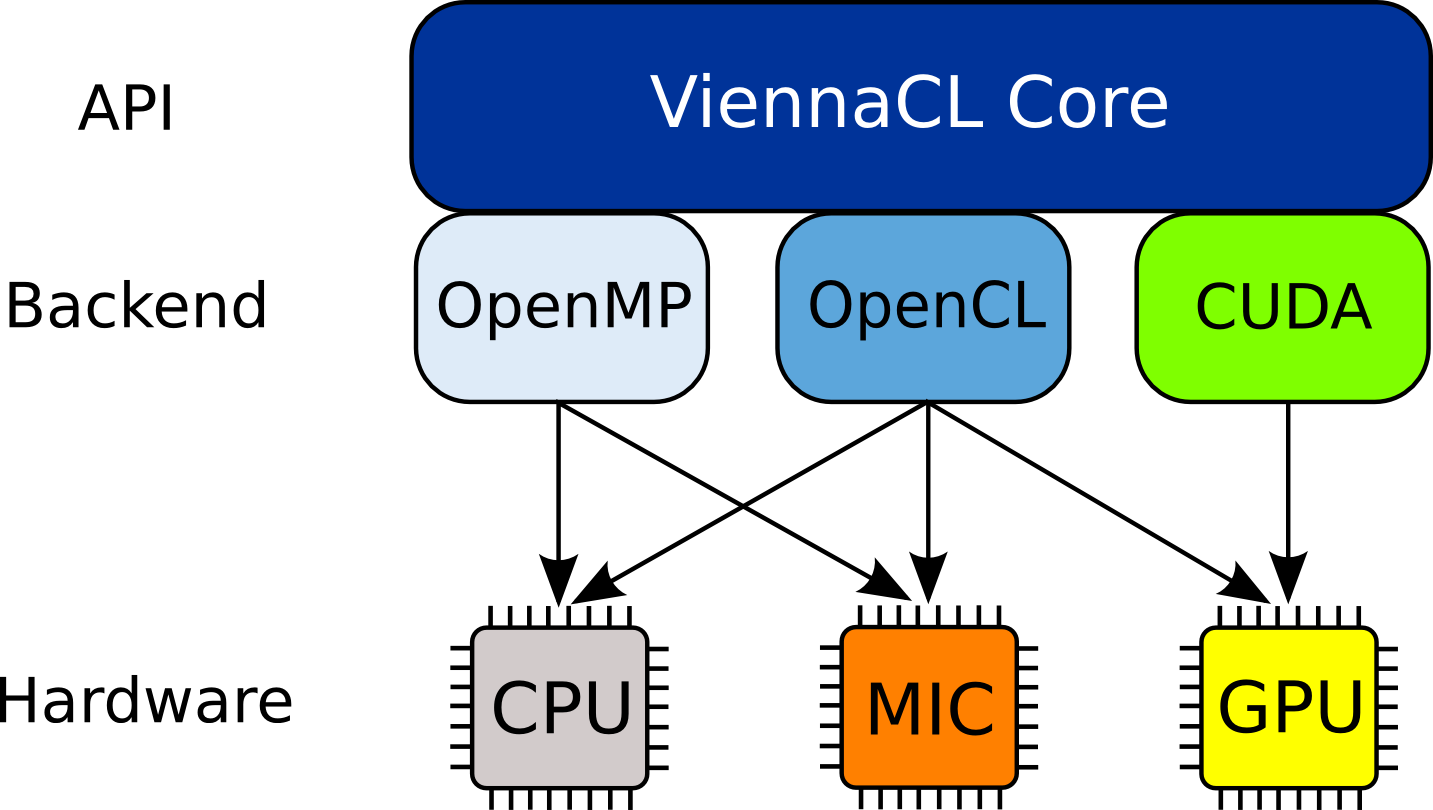
\includegraphics[width=0.4\textwidth]{figures/ViennaCL-arch.png}
  \end{flushright}

  \vspace*{-0.7cm}
  \begin{block}{Dissemination}
    \begin{itemize}
     \item Free Open-Source MIT (X11) License
     \item http://viennacl.sourceforge.net/
     \item 50-100 downloads per week
    \end{itemize}   
  \end{block}

  \begin{block}{Design Rules}
   \begin{itemize}
    \item Reasonable default values
    \item Compatible to Boost.uBLAS whenever possible 
    \item In doubt: clean design over performance
   \end{itemize}
  \end{block}

\end{frame}



\begin{frame}[fragile]
\frametitle{About ViennaCL}

 \begin{block}{Basic Types}
   \begin{itemize}
    \item scalar, vector
    \item matrix, compressed\_matrix, coordinate\_matrix, ell\_matrix, hyb\_matrix
   \end{itemize}
 \end{block}

 \begin{block}{Data Initialization}
    \begin{itemize}
    \item  { 
  \begin{lstlisting}
     std::vector<double>      std_x(100);
   ublas::vector<double>    ublas_x(100);
viennacl::vector<double>      vcl_x(100);

for (size_t i=0; i<100; ++i)
  //   std_x[i] = rand();  // (1)
  // ublas_x[i] = rand();  // (2)
       vcl_x[i] = rand();  // (3)

  \end{lstlisting} }
    \item (3) is fastest, right?
%   \item Reuse of C++ STL coding conventions
 \end{itemize}

 \end{block}
\end{frame}





\begin{frame}[fragile]
\frametitle{About ViennaCL}

 \begin{block}{Basic Types}
   \begin{itemize}
    \item scalar, vector
    \item matrix, compressed\_matrix, coordinate\_matrix, ell\_matrix, hyb\_matrix
   \end{itemize}
 \end{block}

 \begin{block}{Data Initialization}
    \begin{itemize}
     \item Using viennacl::copy() 
    \item  { 
  \begin{lstlisting}
     std::vector<double>      std_x(100);
   ublas::vector<double>    ublas_x(100);
viennacl::vector<double>      vcl_x(100);

/* setup of std_x and ublas_x omitted */

viennacl::copy(std_x.begin(), std_x.end(),
               vcl_x.begin());   //to GPU
viennacl::copy(vcl_x.begin(), vcl_x.end(),
               ublas_x.begin()); //to CPU
  \end{lstlisting} }

 \end{itemize}

 \end{block}
\end{frame}


\begin{frame}[fragile]
\frametitle{About ViennaCL}

 \begin{block}{Basic Types}
   \begin{itemize}
    \item scalar, vector
    \item matrix, compressed\_matrix, coordinate\_matrix, ell\_matrix, hyb\_matrix
   \end{itemize}
 \end{block}

 \begin{block}{Data Initialization}
    \begin{itemize}
     \item Using viennacl::copy() 
    \item  { 
  \begin{lstlisting}
     std::vector<std::vector<double> >    std_A;
   ublas::matrix<double>                ublas_A;
viennacl::matrix<double>                  vcl_A;

/* setup of std_A and ublas_A omitted */

viennacl::copy(std_A, vcl_A);    // CPU to GPU
viennacl::copy(vcl_A, ublas_A);  // GPU to CPU
  \end{lstlisting} }
    \item Iterator concept doesn't quite work on accelerators
 \end{itemize}

 \end{block}
\end{frame}




\begin{frame}[fragile]
\frametitle{Internals}

 \begin{block}{Vector Addition}
  \begin{lstlisting}
 x = y + z;
  \end{lstlisting}
  
  \begin{itemize}
   \item Temporaries are costly (particularly on GPUs)
  \end{itemize}

 \end{block}


 \begin{block}{Expression Templates}
  \begin{itemize}
   \item Limited expansion
   \item Map to a set of predefined kernels
  \end{itemize}
  
  \begin{lstlisting}
 vector_expression<vector<T>, op_plus, vector<T> >
 operator+(vector<T> & v, vector<T> & w) { ... }

 vector::operator=(vector_expression<...> const & e) {
   viennacl::linalg::avbv(*this, 1,e.lhs(), 1,e.rhs());
 }
  \end{lstlisting}
  \vspace*{0.5cm}

 \end{block}

\end{frame}





%%%%%%%%%%%%%%%%%%%%%%%%%%%%


%% Benchmarks




%\begin{frame}{Benchmarks}
%  \begin{center}
%   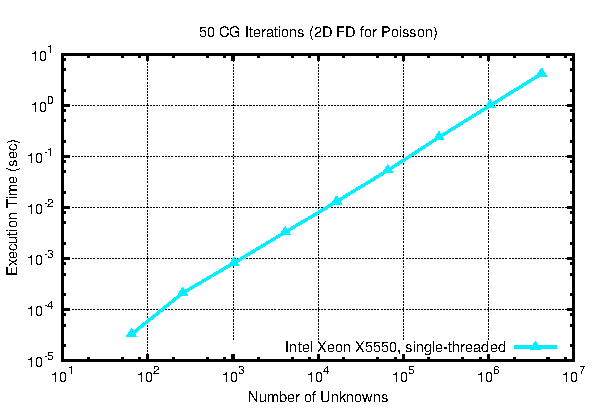
\includegraphics[width=0.95\textwidth]{figures/cg-timings-1}
%  \end{center}
%\end{frame}

%\begin{frame}{Benchmarks}
%  \begin{center}
%   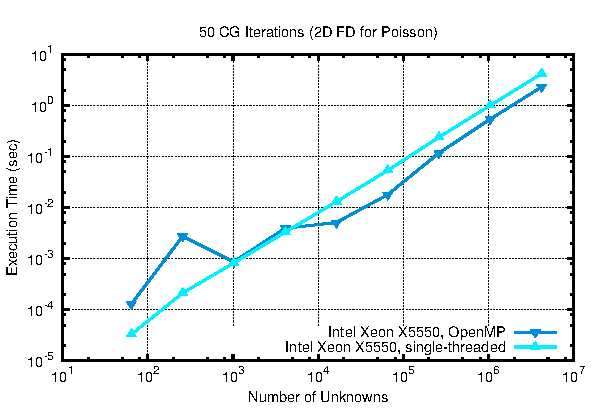
\includegraphics[width=0.95\textwidth]{figures/cg-timings-2}
%  \end{center}
%\end{frame}

%\begin{frame}{Benchmarks}
%  \begin{center}
%   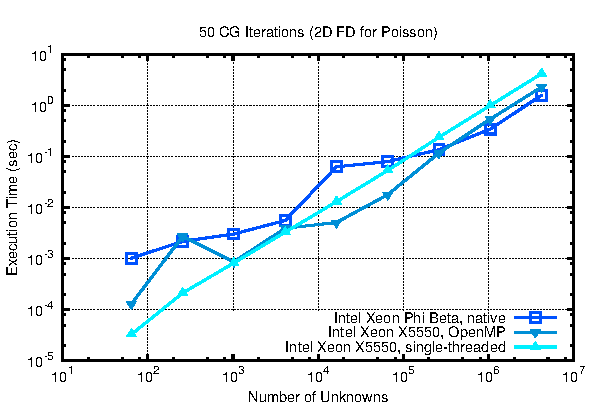
\includegraphics[width=0.95\textwidth]{figures/cg-timings-3}
%  \end{center}
%\end{frame}

%\begin{frame}{Benchmarks}
%  \begin{center}
%   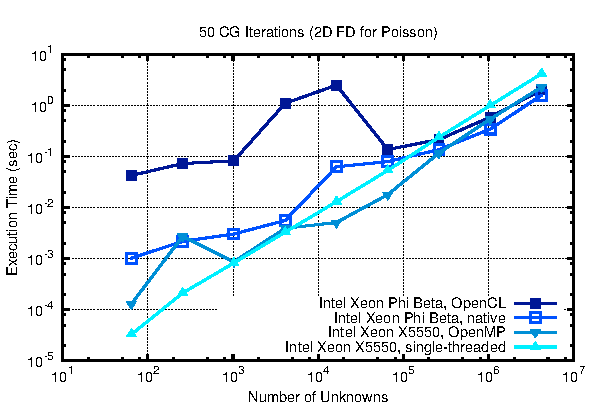
\includegraphics[width=0.95\textwidth]{figures/cg-timings-4}
%  \end{center}
%\end{frame}

%\begin{frame}{Benchmarks}
%  \begin{center}
%   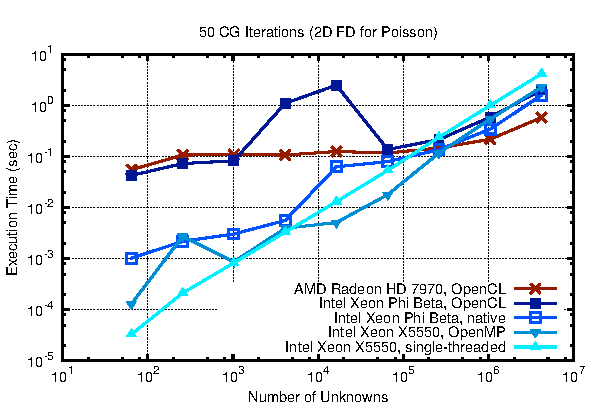
\includegraphics[width=0.95\textwidth]{figures/cg-timings-5}
%  \end{center}
%\end{frame}

%\begin{frame}{Benchmarks}
%  \begin{center}
%   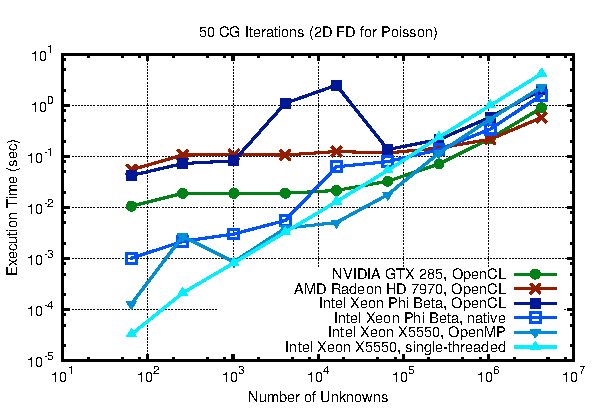
\includegraphics[width=0.95\textwidth]{figures/cg-timings-6}
%  \end{center}
%\end{frame}

\begin{frame}{Benchmarks}
  \begin{center}
   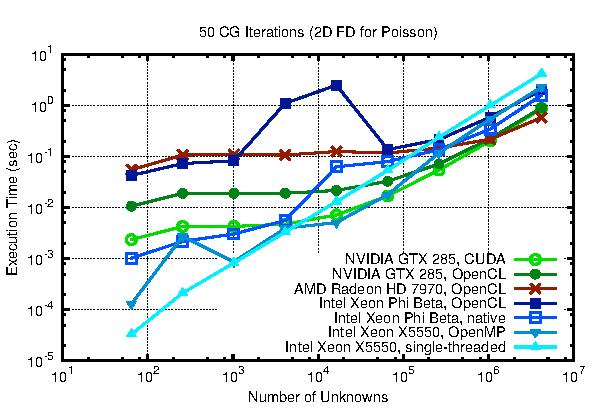
\includegraphics[width=0.95\textwidth]{figures/cg-timings-7}
  \end{center}
\end{frame}





\begin{frame}{Benchmarks}

 \begin{block}{Matrix-Matrix Multiplication}
  \begin{itemize}
   \item Autotuning environment 
   \item 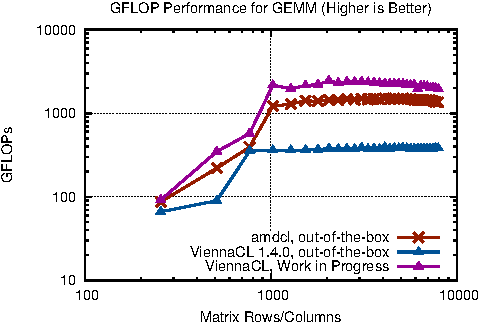
\includegraphics[width=0.85\textwidth]{figures/gemm3.pdf}
   \item \centering (AMD Radeon HD 7970, single precision)
  \end{itemize}

 \end{block}

\end{frame}





%% Acknowledgments and Summary




\begin{frame}{Acknowledgements}

 \begin{minipage}{0.5\textwidth}
  \begin{block}{Contributors}
    \begin{itemize}
     \item Thomas Bertani
     \item Evan Bollig
     \item Philipp Grabenweger
     \item Volodymyr Kysenko
     \item Nikolay Lukash
     \item G\"unther Mader
     \item Vittorio Patriarca
     \item Florian Rudolf
     \item Astrid Rupp
     \item Philippe Tillet
     \item Markus Wagner
     \item Josef Weinbub
     \item Michael Wild
    \end{itemize}
  \end{block}
 \end{minipage}
 \begin{minipage}{0.4\textwidth}
  
\includegraphics[width=0.65\textwidth]{figures/gsoc2011.png}
  \vspace*{0.2cm} \\
  
\includegraphics[width=0.65\textwidth]{figures/gsoc2012.png}
  \vspace*{0.2cm} \\
  
\includegraphics[width=0.65\textwidth]{figures/nvidia_logo_black.png}
  \vspace*{0.2cm} \\
  
\includegraphics[width=0.65\textwidth]{figures/amd-logo.png}
 \end{minipage}

\end{frame}





\begin{frame}{Summary}
 
 \begin{block}{High-Level C++ Approach of ViennaCL}
  \begin{itemize}
   \item Convenience of single-threaded high-level libraries (Boost.uBLAS)
   \item Header-only library for simple integration into existing code
   \item MIT (X11) license
   \item \centering http://viennacl.sourceforge.net/
  \end{itemize}
 \end{block}

 \begin{block}{Selected Features}
  \begin{itemize}
   \item Backends: OpenMP, OpenCL, CUDA
   \item Iterative Solvers: CG, BiCGStab, GMRES
   \item Preconditioners: AMG, SPAI, ILU, Jacobi
   \item BLAS: Levels 1-3
   \item 
  \end{itemize}
 \end{block}

\end{frame}



\begin{frame}{Part 2}
 \begin{center}
   \Huge PETSc \\[2em] \large Portable Extensible Toolkit for Scientific Computing
 \end{center}
\end{frame}



\begin{frame}[fragile]
\frametitle{PETSc}
 \begin{block}{Obtaining PETSc}
 \begin{itemize}
  \item Linux Package Managers
  \item Web: http://mcs.anl.gov/petsc, download tarball
  \item Git: https://bitbucket.org/petsc/petsc
  \item Mercurial: https://bitbucket.org/petsc/petsc-hg
 \end{itemize}
 \end{block}

 \begin{block}{Installing PETSc}
 \begin{itemize}
  \item
 \begin{lstlisting}[escapechar={@}]
$> cd /path/to/petsc/workdir
$> git clone \
     https:@/@/bitbucket.org/petsc/petsc.git \
     --branch master --depth 1
$> cd petsc
 \end{lstlisting}
  \item
 \begin{lstlisting}
$> export PETSC_DIR=$PWD PETSC_ARCH=mpich-gcc-dbg
$> ./configure --with-cc=gcc --with-fc=gfortran 
                 --download-f-blas-lapack
                 --download-{mpich,ml,hypre}
\end{lstlisting}
 \end{itemize}
 \end{block}

\end{frame}


\begin{frame}{PETSc}
\vspace*{-0.2cm}
\begin{center} {\bf Portable} Extensible Toolkit for Scientific Computing \end{center}
\vspace*{-0.2cm}
\begin{block}{Architecture}
    \begin{itemize}  \vspace*{-0.2cm}
    \item tightly coupled (e.g. XT5, BG/P, Earth Simulator)
    \item loosely coupled such as network of workstations
    \item GPU clusters (many vector and sparse matrix kernels)
    \end{itemize}
\end{block} \vspace*{-0.2cm}

\begin{block}{Software Environment}
  \begin{itemize}\vspace*{-0.2cm}
   \item Operating systems (Linux, Mac, Windows, BSD, proprietary Unix)
   \item Any compiler
   \item Usable from C, C++, Fortran 77/90, Python, and MATLAB
   \item Real/complex, single/double/quad precision, 32/64-bit int
  \end{itemize}
\end{block}\vspace*{-0.2cm}

\begin{block}{System Size}
  \begin{itemize}\vspace*{-0.2cm}
   \item 500B unknowns, 75\% weak scalability on Jaguar (225k cores) \\
    and Jugene (295k cores)
   \item Same code runs performantly on a laptop
  \end{itemize}
\end{block}\vspace*{-0.2cm}


\begin{block}{Free to everyone (BSD-style license), open development}\end{block} \vspace*{-0.4cm}

\end{frame}


\begin{frame}{PETSc}

\begin{center}Portable {\bf Extensible} Toolkit for Scientific Computing \end{center}

\begin{block}{Philosophy: Everything has a plugin architecture}
\begin{itemize}
  \item Vectors, Matrices, Coloring/ordering/partitioning algorithms
  \item Preconditioners, Krylov accelerators
  \item Nonlinear solvers, Time integrators
  \item Spatial discretizations/topology$^*$
\end{itemize}

\end{block}

\begin{block}{Example}
  \begin{itemize}
   \item Vendor supplies matrix format and associated preconditioner, distributes
	compiled shared library.  
   \item Application user loads plugin at runtime, no source
	code in sight.
  \end{itemize}
\end{block}

 \vspace{2cm}
\end{frame}


\begin{frame}{PETSc}

\begin{center} Portable Extensible {\bf Toolkit} for Scientific Computing \end{center}

\begin{block}{Toolset}
  \begin{itemize}
   \item algorithms
   \item (parallel) debugging aids
   \item low-overhead profiling
  \end{itemize}
\end{block}

\begin{block}{Composability}
 \begin{itemize}
  \item try new algorithms by choosing from product space
  \item composing existing algorithms (multilevel, domain decomposition, splitting)
 \end{itemize}
\end{block}

\begin{block}{Experimentation}
\begin{itemize}
  \item Impossible to pick the solver \emph{a priori}
  \item PETSc's response: expose an algebra of composition
  \item keep solvers decoupled from physics and discretization
\end{itemize}
\end{block}
\end{frame}

\begin{frame}{PETSc}
\vspace*{-0.2cm}
\begin{center}
 Portable Extensible Toolkit for {\bf Scientific Computing}
\end{center}
\vspace*{-0.2cm}

  \begin{block}{Computational Scientists}
    \begin{itemize}\vspace*{-0.2cm}
    \item PyLith (CIG), Underworld (Monash), Magma Dynamics (LDEO, Columbia), PFLOTRAN (DOE), SHARP/UNIC (DOE)
    \end{itemize}
  \end{block}\vspace*{-0.2cm}
  
  \begin{block}{ Algorithm Developers (iterative methods and preconditioning)} \end{block}\vspace*{-0.4cm}
  
  \begin{block}{ Package Developers}
    \begin{itemize} \vspace*{-0.2cm}
    \item SLEPc, TAO, Deal.II, Libmesh, FEniCS, PETSc-FEM, MagPar, OOFEM, FreeCFD, OpenFVM
    \end{itemize}
  \end{block}\vspace*{-0.2cm}
  
  \begin{block}{Funding}
    \begin{itemize} \vspace*{-0.2cm}    
      \item Department of Energy
      \begin{itemize}\item SciDAC, ASCR ISICLES, MICS Program, INL Reactor Program
      \end{itemize}
    \item National Science Foundation
      \begin{itemize}\item CIG, CISE, Multidisciplinary Challenge Program
      \end{itemize}
    \end{itemize}
  \end{block}\vspace*{-0.2cm}
  
  \begin{block}{Documentation and Support}
   \begin{itemize}\vspace*{-0.2cm}
    \item Hundreds of tutorial-style examples
    \item Hyperlinked manual, examples, and manual pages for all routines
    \item Support from \url{petsc-maint@mcs.anl.gov}
   \end{itemize}
  \end{block}
  
\end{frame}

\begin{frame}[fragile]
\frametitle{Flow Control for a PETSc Application}

\begin{center}
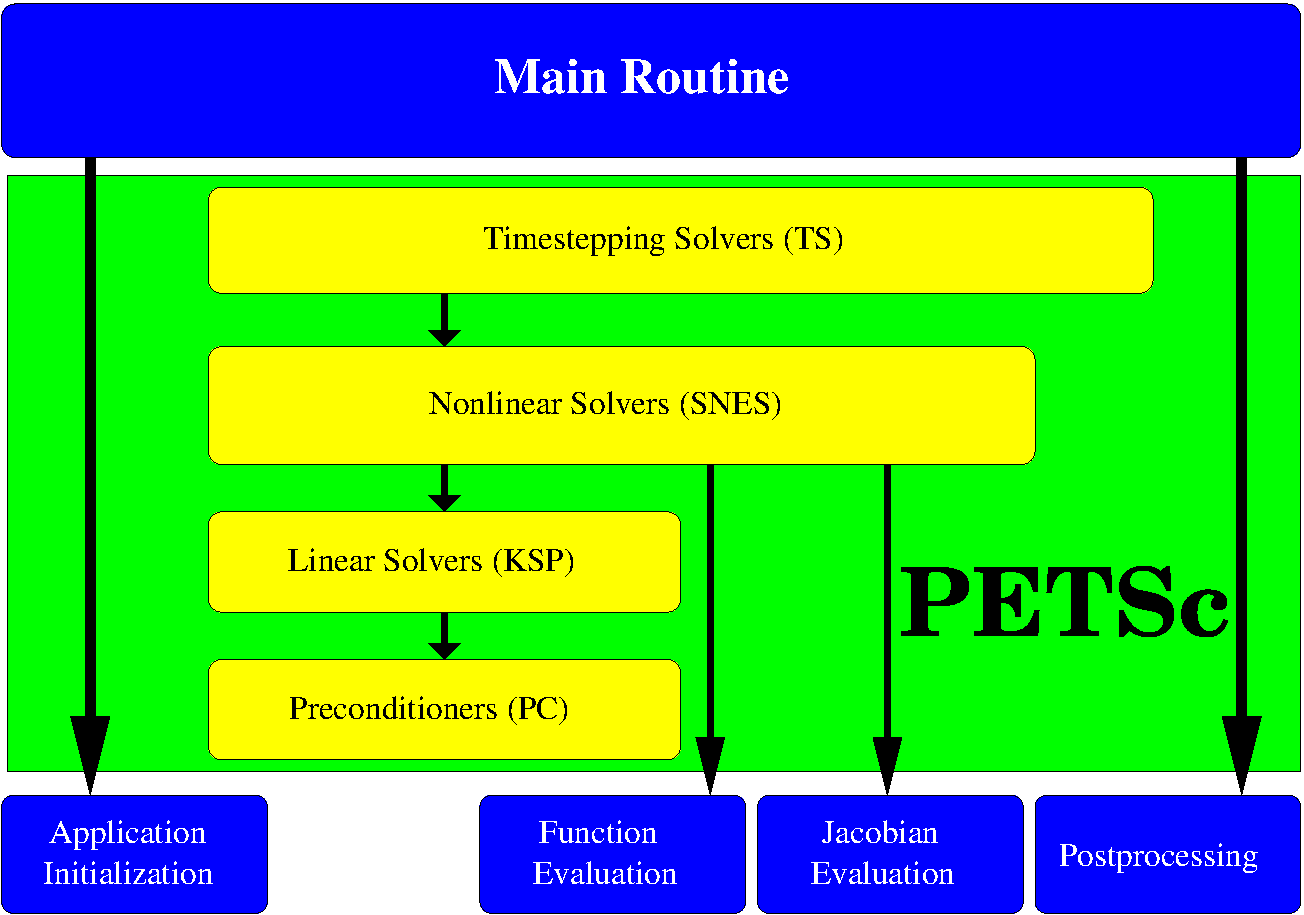
\includegraphics[width=4.0in]{figures/FlowControl}
\end{center}
\end{frame}


\begin{frame}[fragile]
\frametitle{PETSc Pyramid}
 \begin{block}{PETSc Structure} \vspace{0.3cm}
   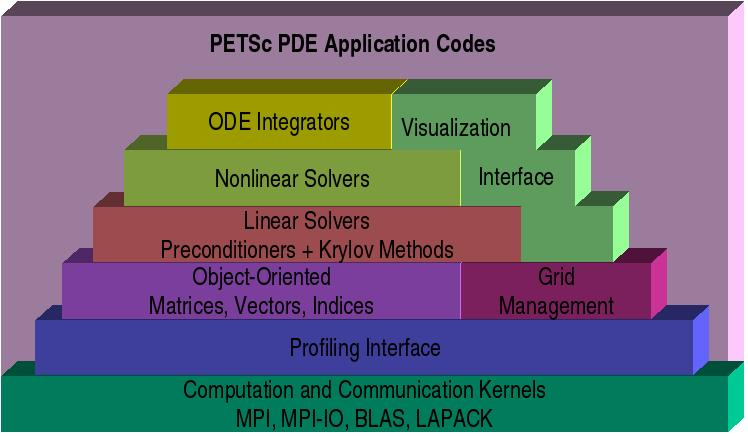
\includegraphics[width=1.0\textwidth]{PETScPyramid.jpg}
 \end{block}

\end{frame}




\begin{frame}
\frametitle{Ghost Values}

\begin{block}{To evaluate a local function $f(x)$, each process requires}
\begin{itemize}
  \item its local portion of the vector $x$
  \item its {\color{cyan}ghost values}, bordering portions of $x$ owned by neighboring processes
\end{itemize}
\end{block}

\begin{center}
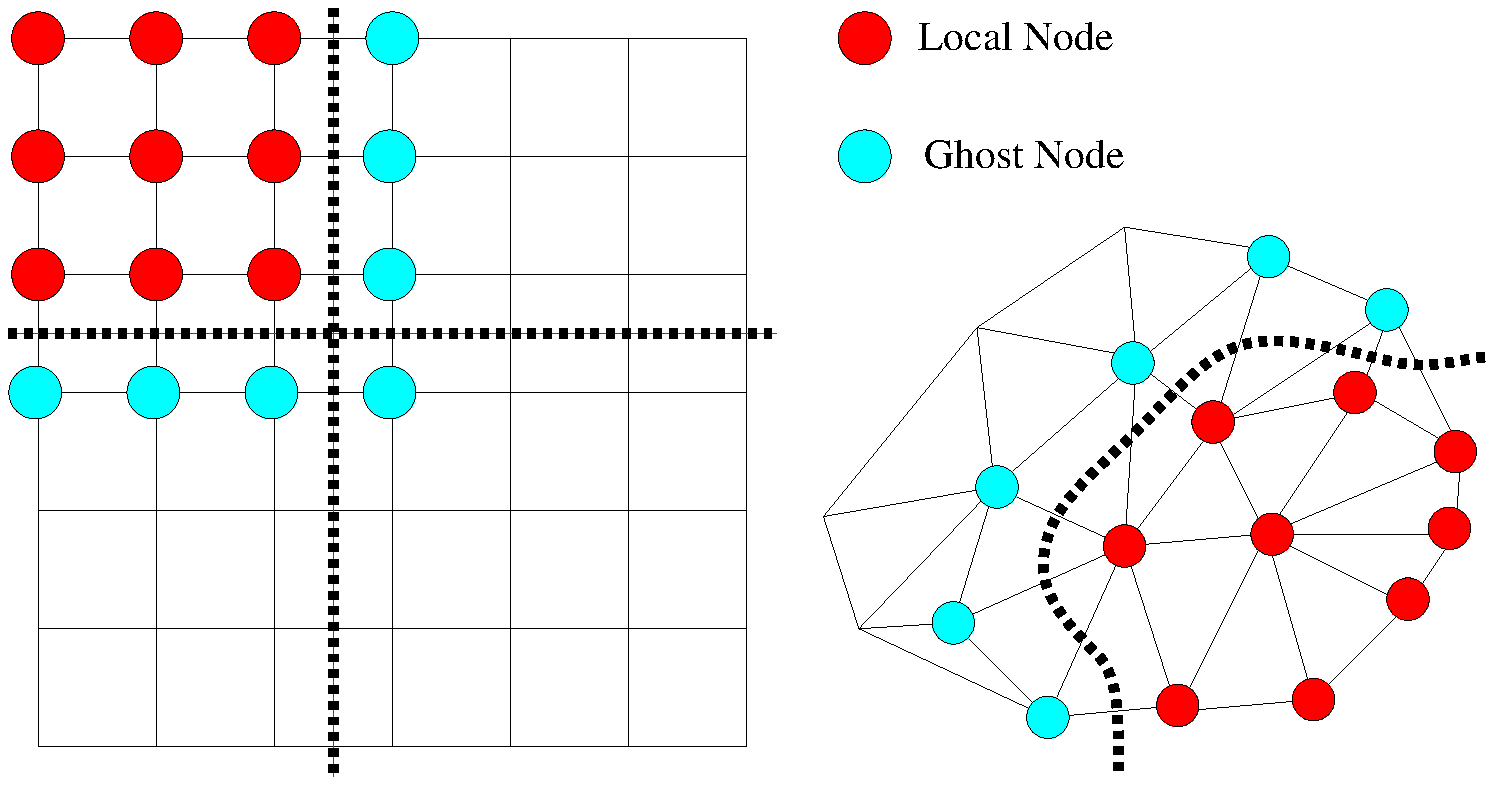
\includegraphics[width=4in]{figures/GhostValues}
\end{center}

\end{frame}

\begin{frame}{DMDA Global Numberings}

\begin{center}
\begin{tabular}{cc}
\begin{tabular}{c}
\begin{tabular}{|ccc|cc|}
\hline
\multicolumn{3}{|c|}{Proc 2} & \multicolumn{2}{c|}{Proc 3} \\
\hline
25 & 26 & 27 & 28 & 29 \\
20 & 21 & 22 & 23 & 24 \\
15 & 16 & 17 & 18 & 19 \\
\hline
10 & 11 & 12 & 13 & 14 \\
 5 &  6 &  7 &  8 &  9 \\
 0 &  1 &  2 &  3 &  4 \\
\hline
\multicolumn{3}{|c|}{Proc 0} & \multicolumn{2}{c|}{Proc 1} \\
\hline
\end{tabular} \\
Natural numbering
\end{tabular}
& 
\begin{tabular}{c}
\begin{tabular}{|ccc|cc|}
\hline
\multicolumn{3}{|c|}{Proc 2} & \multicolumn{2}{c|}{Proc 3} \\
\hline
21 & 22 & 23 & 28 & 29 \\
18 & 19 & 20 & 26 & 27 \\
15 & 16 & 17 & 24 & 25 \\
\hline
 6 &  7 &  8 & 13 & 14 \\
 3 &  4 &  5 & 11 & 12 \\
 0 &  1 &  2 &  9 & 10 \\
\hline
\multicolumn{3}{|c|}{Proc 0} & \multicolumn{2}{c|}{Proc 1} \\
\hline
\end{tabular}\\
PETSc numbering
\end{tabular}
\end{tabular}
\end{center}
\end{frame}

\begin{frame}{DMDA Global vs. Local Numbering}

\begin{itemize}
  \item {\bf Global}: Each vertex has a unique id, belongs on a unique process

  \item {\bf Local}: Numbering includes vertices from neighboring processes
  \begin{itemize}
    \item These are called {\color{cyan}ghost} vertices
  \end{itemize}
\end{itemize}

\begin{center}
\begin{tabular}{cc}
\begin{tabular}{c}
\begin{tabular}{|ccc|cc|}
\hline
\multicolumn{3}{|c|}{Proc 2} & \multicolumn{2}{c|}{Proc 3} \\
\hline
 X &  X &  X &  X &  X \\
 X &  X &  X &  X &  X \\
{\color{cyan}12} & {\color{cyan}13} & {\color{cyan}14} & {\color{cyan}15} &  X \\
\hline
 8 &  9 & 10 & {\color{cyan}11} &  X \\
 4 &  5 &  6 & {\color{cyan}7} &  X \\
 0 &  1 &  2 & {\color{cyan}3} &  X \\
\hline
\multicolumn{3}{|c|}{Proc 0} & \multicolumn{2}{c|}{Proc 1} \\
\hline
\end{tabular} \\
Local numbering
\end{tabular}
& 
\begin{tabular}{c}
\begin{tabular}{|ccc|cc|}
\hline
\multicolumn{3}{|c|}{Proc 2} & \multicolumn{2}{c|}{Proc 3} \\
\hline
21 & 22 & 23 & 28 & 29 \\
18 & 19 & 20 & 26 & 27 \\
15 & 16 & 17 & 24 & 25 \\
\hline
 6 &  7 &  8 & 13 & 14 \\
 3 &  4 &  5 & 11 & 12 \\
 0 &  1 &  2 &  9 & 10 \\
\hline
\multicolumn{3}{|c|}{Proc 0} & \multicolumn{2}{c|}{Proc 1} \\
\hline
\end{tabular}\\
Global numbering
\end{tabular}
\end{tabular}
\end{center}
\end{frame}

\begin{frame}[fragile]{Working with the Local Form}

\begin{block}{Wouldn't it be nice if we could just write our code for the natural numbering?}
 
 \only<1>{
\begin{center}
\begin{tabular}{cc}
\begin{tabular}{c}
\begin{tabular}{|ccc|cc|}
\hline
\multicolumn{3}{|c|}{Proc 2} & \multicolumn{2}{c|}{Proc 3} \\
\hline
25 & 26 & 27 & 28 & 29 \\
20 & 21 & 22 & 23 & 24 \\
15 & 16 & 17 & 18 & 19 \\
\hline
10 & 11 & 12 & 13 & 14 \\
 5 &  6 &  7 &  8 &  9 \\
 0 &  1 &  2 &  3 &  4 \\
\hline
\multicolumn{3}{|c|}{Proc 0} & \multicolumn{2}{c|}{Proc 1} \\
\hline
\end{tabular} \\
Natural numbering
\end{tabular}
& 
\begin{tabular}{c}
\begin{tabular}{|ccc|cc|}
\hline
\multicolumn{3}{|c|}{Proc 2} & \multicolumn{2}{c|}{Proc 3} \\
\hline
21 & 22 & 23 & 28 & 29 \\
18 & 19 & 20 & 26 & 27 \\
15 & 16 & 17 & 24 & 25 \\
\hline
 6 &  7 &  8 & 13 & 14 \\
 3 &  4 &  5 & 11 & 12 \\
 0 &  1 &  2 &  9 & 10 \\
\hline
\multicolumn{3}{|c|}{Proc 0} & \multicolumn{2}{c|}{Proc 1} \\
\hline
\end{tabular}\\
PETSc numbering
\end{tabular}
\end{tabular}
\end{center}
\vspace*{1cm}
    }
    
    
 \only<2>{
  \begin{itemize}
  \item Yes, that's what \lstinline|DMDAVecGetArray()| is for.
  \end{itemize}
  }
  
  \end{block}
  
  \only<2>{
 \begin{block}{DMDA offers \emph{local} callback functions}
    \begin{itemize}
      \item \lstinline|FormFunctionLocal()|, set by \lstinline|DMDASetLocalFunction()|
      \item \lstinline|FormJacobianLocal()|, set by \lstinline|DMDASetLocalJacobian()|
    \end{itemize}
 \end{block}

 
 \begin{block}{Evaluating the nonlinear residual $F(x)$}
    \begin{itemize}
      \item Each process evaluates the local residual
      \item PETSc assembles the global residual automatically
        \begin{itemize}
        \item Uses \lstinline|DMLocalToGlobal()| method
        \end{itemize}
    \end{itemize}
 \end{block}
 }

\end{frame}


%%%%%%%%%  Go to p-Bratu





\begin{frame}{The $\mathfrak{p}$-Bratu Equation}

  \begin{block}{The ``Hello World of PDEs''}
  \begin{itemize}
   \item Poisson's Equation
    \begin{equation*}
      -\nabla \cdot \bigl(\nabla u \bigr) = f,
    \end{equation*}
   \item Leads to symmetric, positive definite system matrices
   \item Commonly used in numerical analysis (corner effects, etc.)
  \end{itemize}
  \end{block}

  \begin{block}{More General Form}
  \begin{itemize}
   \item With diffusivity tensor $\eta$:
    \begin{equation*}
      -\nabla \cdot \bigl( \eta \nabla u \bigr) = f,
    \end{equation*}
   \item Typically: $\eta > \delta > 0$
   \item $\eta$ can be discontinous (material boundaries)
   \item Reduced regularity of solution
  \end{itemize}
  \end{block}
  
\end{frame}


\begin{frame}{The $\mathfrak{p}$-Bratu Equation}

  \begin{block}{Additional Volume Term}
  \begin{itemize}
   \item Consider
    \begin{equation*}
      -\nabla \cdot \bigl(\eta \nabla u \bigr) - \lambda e^u - f = 0 \ ,
    \end{equation*}
   \item Canonical nonlinear form
   \item $e^u$ has ``wrong sign'': turning point at $\lambda_{\text{crit}}$
  \end{itemize}
  \end{block}

  \begin{block}{Another Tweak}
  \begin{itemize}
   \item Diffusivity tensor $\eta$ depends on $u$, e.g.:
    \begin{equation*}
      \eta = \frac{1}{2} \vert \nabla u \vert^2,
    \end{equation*}
   \item Singular or degenerate when $\nabla u = 0$.
  \end{itemize}
  \end{block}
  
\end{frame}


% \section{$\pfrak$-Bratu}
\begin{frame}{The $\mathfrak{p}$-Bratu Equation}

  \begin{block}{$\mathfrak{p}$-Bratu Equation}
  \begin{itemize}
  \item 2-dimensional model problem
    \begin{equation*}
      -\nabla \cdot \bigl(\vert\nabla u\vert^{\mathfrak{p}-2} \nabla u \bigr) - \lambda e^u - f = 0, \qquad 1 \le \mathfrak{p} \le \infty, \quad \lambda < \lambda_{\text{crit}}(\mathfrak{p})
    \end{equation*}
    Singular or degenerate when $\nabla u = 0$, turning point at $\lambda_{\text{crit}}$.
  \end{itemize}
  \end{block}
  
  \begin{block}{Regularized Variant}
  \begin{itemize}
  \item Remove singularity of $\eta$ using a parameter $\varepsilon$:
    \begin{gather*}
      -\nabla \cdot (\eta \nabla u) - \lambda e^u - f = 0 \\
      \eta(\gamma) = (\epsilon^2 + \gamma)^{\frac{\mathfrak{p}-2}{2}} \qquad \gamma(u) = \frac{1}{2} \vert\nabla u\vert^2
    \end{gather*}
  \item       Physical interpretation: diffusivity tensor flattened in direction $\nabla u$
  \end{itemize}
  \end{block}
\end{frame}







%
% Conclusion and Wrap-Up
%
\section{Conclusions}
\begin{frame}{Conclusions}
 
 \begin{block}{PETSc Can Help You}
  \begin{itemize}
   \item Solve algebraic and DAE problems in your application area
   \item Rapidly develop efficient parallel code, can start from examples
   \item Develop new solution methods and data structures
   \item Debug and analyze performance
   \item Advice on software design, solution algorithms, and performance
   \item \centering \texttt{petsc-\{users,dev,maint\}@mcs.anl.gov}

  \end{itemize}
 \end{block}

 \begin{block}{You Can Help PETSc}
  \begin{itemize}
   \item report bugs and inconsistencies, or if you think there is a better way
   \item tell us if the documentation is inconsistent or unclear
   \item consider developing new algebraic methods as plugins, contribute if your idea works
  \end{itemize}
 \end{block}

\end{frame}



\end{document}

